% Visual driver derived from the local PGF arrows.meta Arc Barb examples.
\documentclass[border=4pt]{standalone}
\usepackage{tikz}
\usetikzlibrary{arrows.meta}

\begin{document}
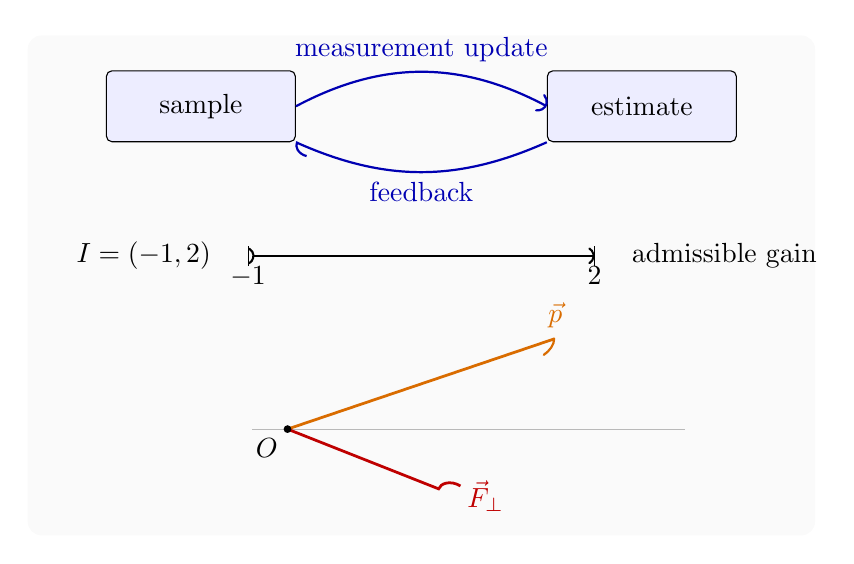
\begin{tikzpicture}[
  state/.style={
    draw,
    rounded corners=2pt,
    minimum width=24mm,
    minimum height=9mm,
    fill=blue!7
  },
  flow/.style={line width=.8pt,blue!70!black},
  vector/.style={line width=1pt,orange!85!black}
]
  \path[fill=gray!4,rounded corners=5pt]
    (-5,-3.1) rectangle (5,3.25);

  % A curved flowchart connection exercises terminal-tangent placement.
  \node[state] (sample) at (-2.8,2.35) {sample};
  \node[state] (estimate) at (2.8,2.35) {estimate};
  \draw[flow,-{Arc Barb[arc=120,length=5pt,width=8pt,round]}]
    (sample.east) to[out=28,in=152]
    node[above] {measurement update} (estimate.west);
  \draw[flow,{Arc Barb[arc=210,length=4.5pt,width=7pt,harpoon,left]}-]
    (sample.south east) to[out=-24,in=-156]
    node[below] {feedback} (estimate.south west);

  % Parenthesis is the source-defined Arc Barb alias for interval ends.
  \node[anchor=east] at (-2.55,.45) {$I=(-1,2)$};
  \draw[line width=.75pt,{Parenthesis[reversed,round]}-{Parenthesis[round]}]
    (-2.2,.45) -- (2.2,.45);
  \draw (-2.2,.32) -- (-2.2,.58) node[below=4pt] {$-1$};
  \draw (2.2,.32) -- (2.2,.58) node[below=4pt] {$2$};
  \node[anchor=west] at (2.55,.45) {admissible gain};

  % Customized one-sided arc barbs form a compact vector inset.
  \coordinate (origin) at (-1.7,-1.75);
  \draw[gray!55] (-2.15,-1.75) -- (3.35,-1.75);
  \draw[vector,-{Arc Barb[
      arc=135,
      length=7pt,
      width=10pt,
      line width=.9pt,
      harpoon,
      right,
      round,
      slant=.3
    ]}]
    (origin) -- ++(3.4,1.15) node[above] {$\vec p$};
  \draw[red!75!black,line width=1pt,-{Arc Barb[
      arc=210,
      length=6pt,
      width=9pt,
      harpoon,
      reversed,
      left
    ]}]
    (origin) -- ++(2.15,-.85) node[right] {$\vec F_{\perp}$};
  \fill (origin) circle (1.4pt);
  \node[below left] at (origin) {$O$};
\end{tikzpicture}
\end{document}
